\documentclass[a4paper,11pt]{report}
\usepackage[T1]{fontenc}
\usepackage[utf8]{inputenc}
\usepackage{lmodern}
\usepackage[francais]{babel}
\usepackage{graphicx}
\usepackage{array}

\title{Data wars }

\author{Guillaume LAROYENNE, Nathan PRETOT \\ Jeremy RENAUD, Tom SALVI, Pierre VALENZA}

\begin{document}

\maketitle
\tableofcontents

\chapter{Introduction}

	\begin{figure}[th]
		\begin{center}
		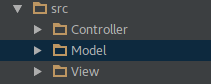
\includegraphics[scale=0.4]{Assets/mvc.png}
      		\caption{Modèle du site \textit{data wars}}
      		\label{fig1}
     		\end{center}
	\end{figure}

	Le site est construit en Modèle-Vue-Controleur. Ainsi l'ensemble des requête SQL se trouve dans la partie Model, les vues des pages du site sont dans la partie View et les fonctions permettant de lié la vue au modèle sont dans la partie Controller.

\chapter{Model}
	Dans le dossier Modele vous trouverez 3 modèles d'où vous pouvez obtenir les informations de la base de donnée utilisé par Data war. Ainsi vous pouvez selectionner, ajouter, modifier et supprimer des informations :

	\begin{figure}[th]
		\begin{center}
		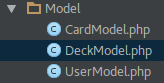
\includegraphics[scale=0.4]{Assets/modele.png}
      		\caption{Modèle du site \textit{data wars}}
      		\label{fig2}
     		\end{center}
	\end{figure}
    
	CardModel contient les requêtes SQL qui sont lié aux \textit{cartes unités et sorts} du jeu.
	DeckModel contient les requêtes SQL qui sont lié aux \textit{decks} du jeu.
	UserModel contient les requêtes SQL qui sont lié aux \textit{comptes} du site.    

\chapter{View}
	\begin{figure}[th]
		\begin{center}
		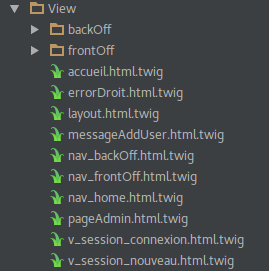
\includegraphics[scale=0.4]{Assets/view.png}
      		\caption{Vue du site \textit{data wars}}
      		\label{fig3}
     		\end{center}
	\end{figure}

	La vue se sépare en 2 sections principales :
	\begin{enumerate}
		\item le backOff
		\item le frontOff
	\end{enumerate}

	Les fichiers en dehors de ces dossiers sont les barres de navigations, la page d'accueil, les pages d'inscription au site et des pages de test.
    
	\section{le backOff}
        Le backOff contient les pages qui ne doivent êtres accessible que par les administrateurs du sites, c'est à partir d'ici que la modifications des cartes et des utilisateurs est possible. \textit{Il est essentiel que ces pages soient accessible seuleument aux administrateurs. }
    \begin{figure}[th]
      \begin{center}
        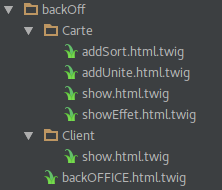
\includegraphics[scale=0.4]{Assets/backOff.png}
        \caption{Zoom sur le bloc grille}
        \label{fig4}
      \end{center}
    \end{figure}

	Comment on peut le voir ci-dessus il existe 2 dossiers :
	\begin{enumerate}
		\item Carte
		\item Client
	\end{enumerate}

	"Carte" contient les pages qui permettent de :
	\begin{enumerate}
		\item addSort : ajouter une carte sort
		\item addUnite : ajouter une carte unité
		\item showEffet : liste les effets de cartes, ajoute un effet
		\item show : liste l'ensemble des cartes présentes dans la base de donnée
	\end{enumerate}

        \subsection{Client}
         Dans le dossier CLient il n'y a qu'une page : "show", elle liste les comptes du site. 
        \begin{figure}[th]
      		\begin{center}
        	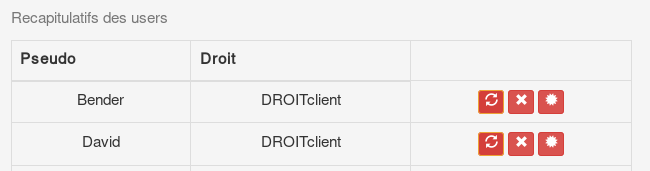
\includegraphics[scale=0.4]{Assets/liste_user.png}
        	\caption{Liste des utilisateurs}
        	\label{fig5}
      		\end{center}
    	\end{figure}

	Ainsi les selon la figure ci-dessus les options disponible, dans l'ordre, sont : 
	\begin{enumerate}
		\item réinitialiser le deck du joueur
		\item supprimer le compte du joueur
		\item le compte obtient les droits administrateurs
	\end{enumerate}
         
	\section{le frontOff}
        Le frontOff contient uniquement une page qui permet au joueur de modifier son deck.
    \begin{figure}[th]
      \begin{center}
        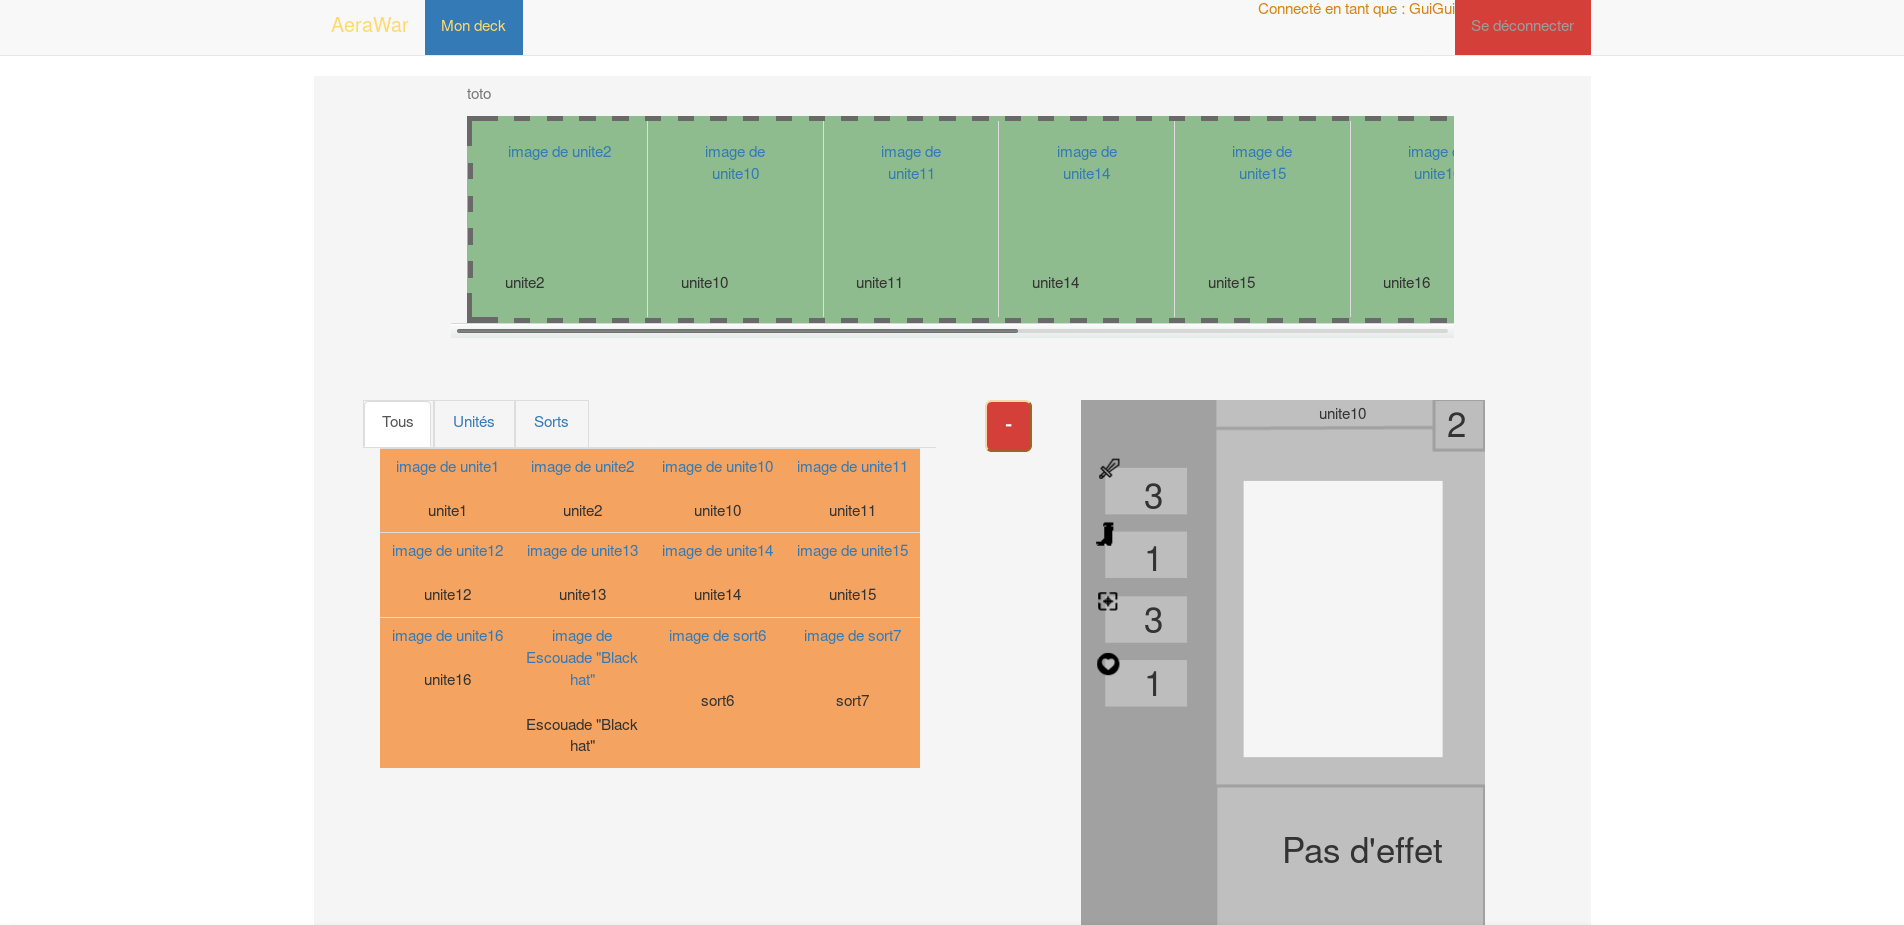
\includegraphics[scale=0.4]{Assets/site.png}
        \caption{Modfication de d'un deck}
        \label{fig6}
      \end{center}
    \end{figure}

	La modification du deck se doit d'être confortable pour l'utilisateur. Ainsi la partie supérieur représente le deck actuel du joueur, le tableau a gauche liste l'ensemble des cartes du jeu et la carte séléctionner s'affiche sur la droite.

\chapter{Controller}
	Dans le dossier Controller vous trouverez l'ensemble des fonctions qui lient la vue avec le modèle.

	\begin{figure}[th]
		\begin{center}
		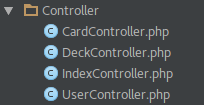
\includegraphics[scale=0.4]{Assets/controller.png}
      		\caption{Modèle du site \textit{data wars}}
      		\label{fig7}
     		\end{center}
	\end{figure}
    
	IndexController contient seulement les actions possible pour un utilisateur non connecter à un compte. Les 3 autres fichiers sont les plus importants :

	\begin{enumerate}
		\item CardController lie les pages qui vont nécessité l'affichage des informations d'une ou plusieurs cartes
		\item DeckController permet toute les actions possible sur un deck
		\item UserController permet toute les actions possible sur un utilisateur
	\end{enumerate}

	\section{le contrôle des données}
        Lorsque des informations sont transmises par l'utilisateur à la base de donnée comme par exemple l'ajout d'une nouvelle carte il est important de procéder aux vérifications des champs de saisie. Silex nous propose de mettre en place des contraintes sur ces champs.
    \begin{figure}[th]
      \begin{center}
        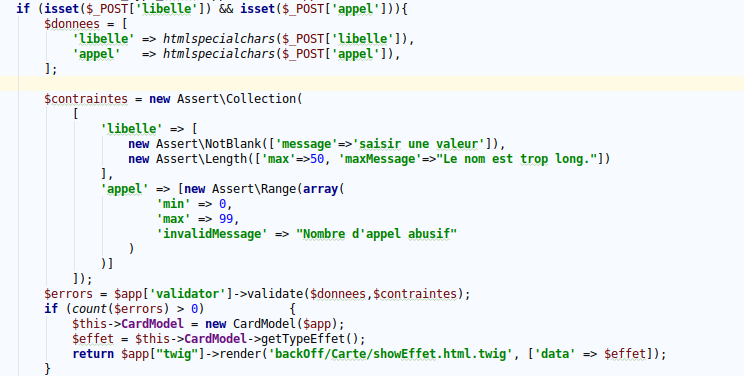
\includegraphics[scale=0.4]{Assets/exemple_contrainte.png}
        \caption{Un exemple de contrainte}
        \label{fig8}
      \end{center}
    \end{figure}

	Comment on peut le voir ci-dessus on peut observer 4 étapes :
	\begin{enumerate}
		\item Récupérer les données entrer
		\item Mettre en place les contraintes
		\item Comparer les données avec les contraintes
		\item Renvoyer le client à la page de saisie si une erreur est présente
	\end{enumerate}

	\section{Appelle des requêtes SQL}
	 \begin{figure}[th]
     		 \begin{center}
        	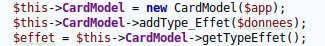
\includegraphics[scale=0.4]{Assets/requete.png}
       		 \caption{Un exemple d'utilisation de requête}
       		 \label{fig9}
     		 \end{center}
   	 \end{figure}
	
	Le code ci-dessus a pour but d'ajouter un effet dans la base de donnée puis de récupérer tout les effets pour enfin les envoyer sur la page "showEffet".

	Voici la procédure a suivre pour utiliser des requêtes SQL et envoyer les données sur la page de retour :
	\begin{enumerate}
		\item Initialiser une variable avec le modèle utiliser
		\item Faites l'appelle des requêtes, le retour peut être stocké dans une variable
		\item Renvoyer l'utilisateur à la page voulu, avec les données si il y en a
	\end{enumerate}
	

        
\end{document}  

